\documentclass[12pt,a4paper]{report}
\usepackage{amsmath}
\usepackage{amsfonts}
\usepackage{amssymb}
\usepackage[utf8]{inputenc}
\usepackage[polish]{babel}
\usepackage[T1]{fontenc}
\usepackage{graphicx}
\usepackage[left=2.5cm,right=1.5cm,top=2cm,bottom=2cm]{geometry}

\begin{document}
\thispagestyle{empty} %usuwanie numeru strony

\includegraphics[scale=0.5]{zut.jpg}
\hfill %rozsuwa grafike

\includegraphics[scale=1.2]{wi.jpg}\\[2cm] %odstep 2cm
\begin{center}
\textbf{\large{Aleksander Przykładowski}}\\[0.5cm]
nr albumu: 123456789\\[0.5cm]
kierunek studiów: Informatyka\\[0.5cm]
specjalność: Systemy komputerowe i oprogramowanie\\[0.5cm]
forma studiów: \textsl{stacjonarne}\\[2cm]
\textbf{{\large}METODY POSZUKIWANIA OPTYMALNYCH ROZWIĄZAŃ}\\[0.5cm]
\textbf{{\large}METHODS OF EXPLORATION FOR OPTIMUM SOLUTIONS}\\[2cm]
praca dyplomowa inżynierska\\[0.5cm]
napisana pod kierunkiem:\\[0.5cm]
\textbf{{\large}prof. dr hab. Jana Niezawodnego}\\[0.5cm]
Katedra Systemów Multimedialnych\\[2cm]
\end{center}
\begin{tabular}{lc}
    \small{Data wydania tematu pracy:}&\small{07.12.2019}\\
    &\\
    \samll{Data dopuszczenia pracy do egzaminu:}&\hdotsfor{}
\end{tabular}
\vspace{2cm}
\begin{center}
Szczecin, 2019    
\end{center}
%%%%%%%%%%%%%%%%%%%%%%%%%%%%%%%%%%%%%%%STRONA - TYTUL ANGIELSKI
\newpage
METHODS OF EXPLORATION FOR OPTIMUM SOLUTIONS\\[2cm]
Streszczenie po angielsku
%%%%%%%%%%%%%%%%%%%%%%%%%%%%%%%%%%%%%%%STROONA - OSWIADCZENIE
\newpage
\vspace*{3cm}
\begin{center}
\textbf{\large{OŚWIADCZENIE\\AUTORA PRACY DYPLOMOWEJ}}    
\end{center}
Oświadczam, że praca dyplomowa inżynierska/magisterska (podać rodzaj pracy) pn.\\
.\dotfill\\
.\dotfill\\
\vspace{-1cm}
\begin{center}
    \small{\textsl{(temat pracy dyplomowej)}}\\
\end{center}
\vspace{-0.5cm}
napisana pod kierunkiem:\\[0.2cm]
.\dotfill\\
\vspace{-1cm}
\begin{center}
    \small{\textsl{(tytuł lub stopień naukowy imię i nazwisko opiekuna pracy)}}
\end{center}
jest w całości moim samodzielnym autorskim opracowaniem sporządzonym przy wykorzystaniu wykazanej w pracy literatury przedmiotu i materiałów źródłowych.\\
Złożona w dziekanacie \textbf{{\large}Wydziału Informatyki}\\[0.5cm]
treść  mojej pracy dyplomowej w formie elektronicznej jest zgodna z treścią w formie pisemnej/pisemnej i graficznej*.\\[0.5cm]
Oświadczam ponadto, że złożona w dziekanacie praca dyplomowa ani jej fragmenty nie były wcześniej przedmiotem procedur procesu dyplomowania związanych z uzyskaniem tytułu zawodowego w uczelniach wyższych.\\[1cm]
\hspace*{11cm}…………………………\\
\hspace*{12cm}podpis dyplomanta
\vspace{1cm}
Szczecin, dn. ………………….

\noindent * niepotrzebne skreślić 
%%%%%%%%%%%%%%%%%%%%%%%%%%%%%%%%%%%%%%%STRONA - SPIS TRESCI
\newpage
\tableofcontents

%%%%%%%%%%%%%%%%%%%%%%%%%%%%%%%%%%%%%%%STRONA - WPROWADZENIE
\newpage
\chapter*{Wprowadzenie}
\addcontentsline{toc}{chapter}{Wprowadzenie}
Cel pracy \\
Zakres pracy
%%%%%%%%%%%%%%%%%%%%%%%%%%%%%%%%%%%%%%%STRONA - ROZDZIAL 1
\newpage
\chapter{Wypunktowania i wyliczenia}
Punkty kontrolne
\begin{itemize}
\item{Jeden}
\item{Dwa} 
\end{itemize}
\begin{list}{*}{Punkty kontrolne}
\item Pierwszy punkt
\item Drugi punkt
\end{list}
%%%%%%%%%%%%%%%%%%%%%%%%%%%%%%%%%%%%%%%STRONA - ROZDZIAL 2
\newpage
\chapter{Tabele}
Tabelka do wyswietlania\\
\begin{table}[h]
    \centering
    \caption{Jakaś tabelka}
    \begin{tabular}{|r|c|c|c|c|}
    \hline
        Jakieś wartości &1&2&3&4\\
        \hline
        Inne wartości &5&6&7&8\\ 
        \hline
        Jeszcze inne &9&10&11&12\\
        \hline
    \end{tabular}
 \end{table}
 \begin{table}[h]
    \centering
    \caption{Jakaś druga tabelka}
    \begin{tabular}{|r|c|c|c|c|}
    \hline
        Jakieś wartości &\multicolumn{2}{c|}{2+2}&3&4\\
        \hline
        Inne wartości &5&\multicolumn{3}{c|}{2+2}\\ 
        \hline
        Jeszcze inne &9&10&11&12\\
        \hline
    \end{tabular}
 \end{table}
%%%%%%%%%%%%%%%%%%%%%%%%%%%%%%%%%%%%%%%STRONA - ROZDZIAL 3
\newpage
\chapter{Wzory matematyczne}
Działania matematyczne: \\[1cm]
\begin{math}
x^{2y}\\
log_2\\
x^{y}_{1}\\[1cm]
Wielokropki\\[1cm]
\ldots
\cdots
\vdots
\ddots\\[1cm] 
Inne\\[1cm]
\frac{(x+y)^2}{2x+b^2}\\[0.5cm]
\sqrt[3]{20}\\[0.5cm]
(a+b)^2 = a^2+2ab+b^2\\[0.5cm]
\lim_{x\rightarrow 0}\\[0.5cm]
\left\{\begin{array}{ccl}
     y&=&2x+3  \\
     y&=&3c-4
\end{array}\right
\end{math}
%%%%%%%%%%%%%%%%%%%%%%%%%%%%%%%%%%%%%%%STRONA - ROZDZIAL 4
\newpage
\chapter{Rysunki i schematy}
Rysunek \\[1cm]
\begin{figure}[h]
    \centering
    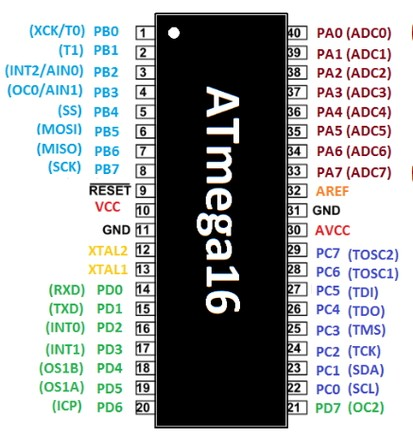
\includegraphics[scale=2]{atmega16.jpg}
    \caption{Atmega}
    \label{fig:my_label}
\end{figure}
Schemat \\[1cm]
\begin{figure}[h]
    \centering
    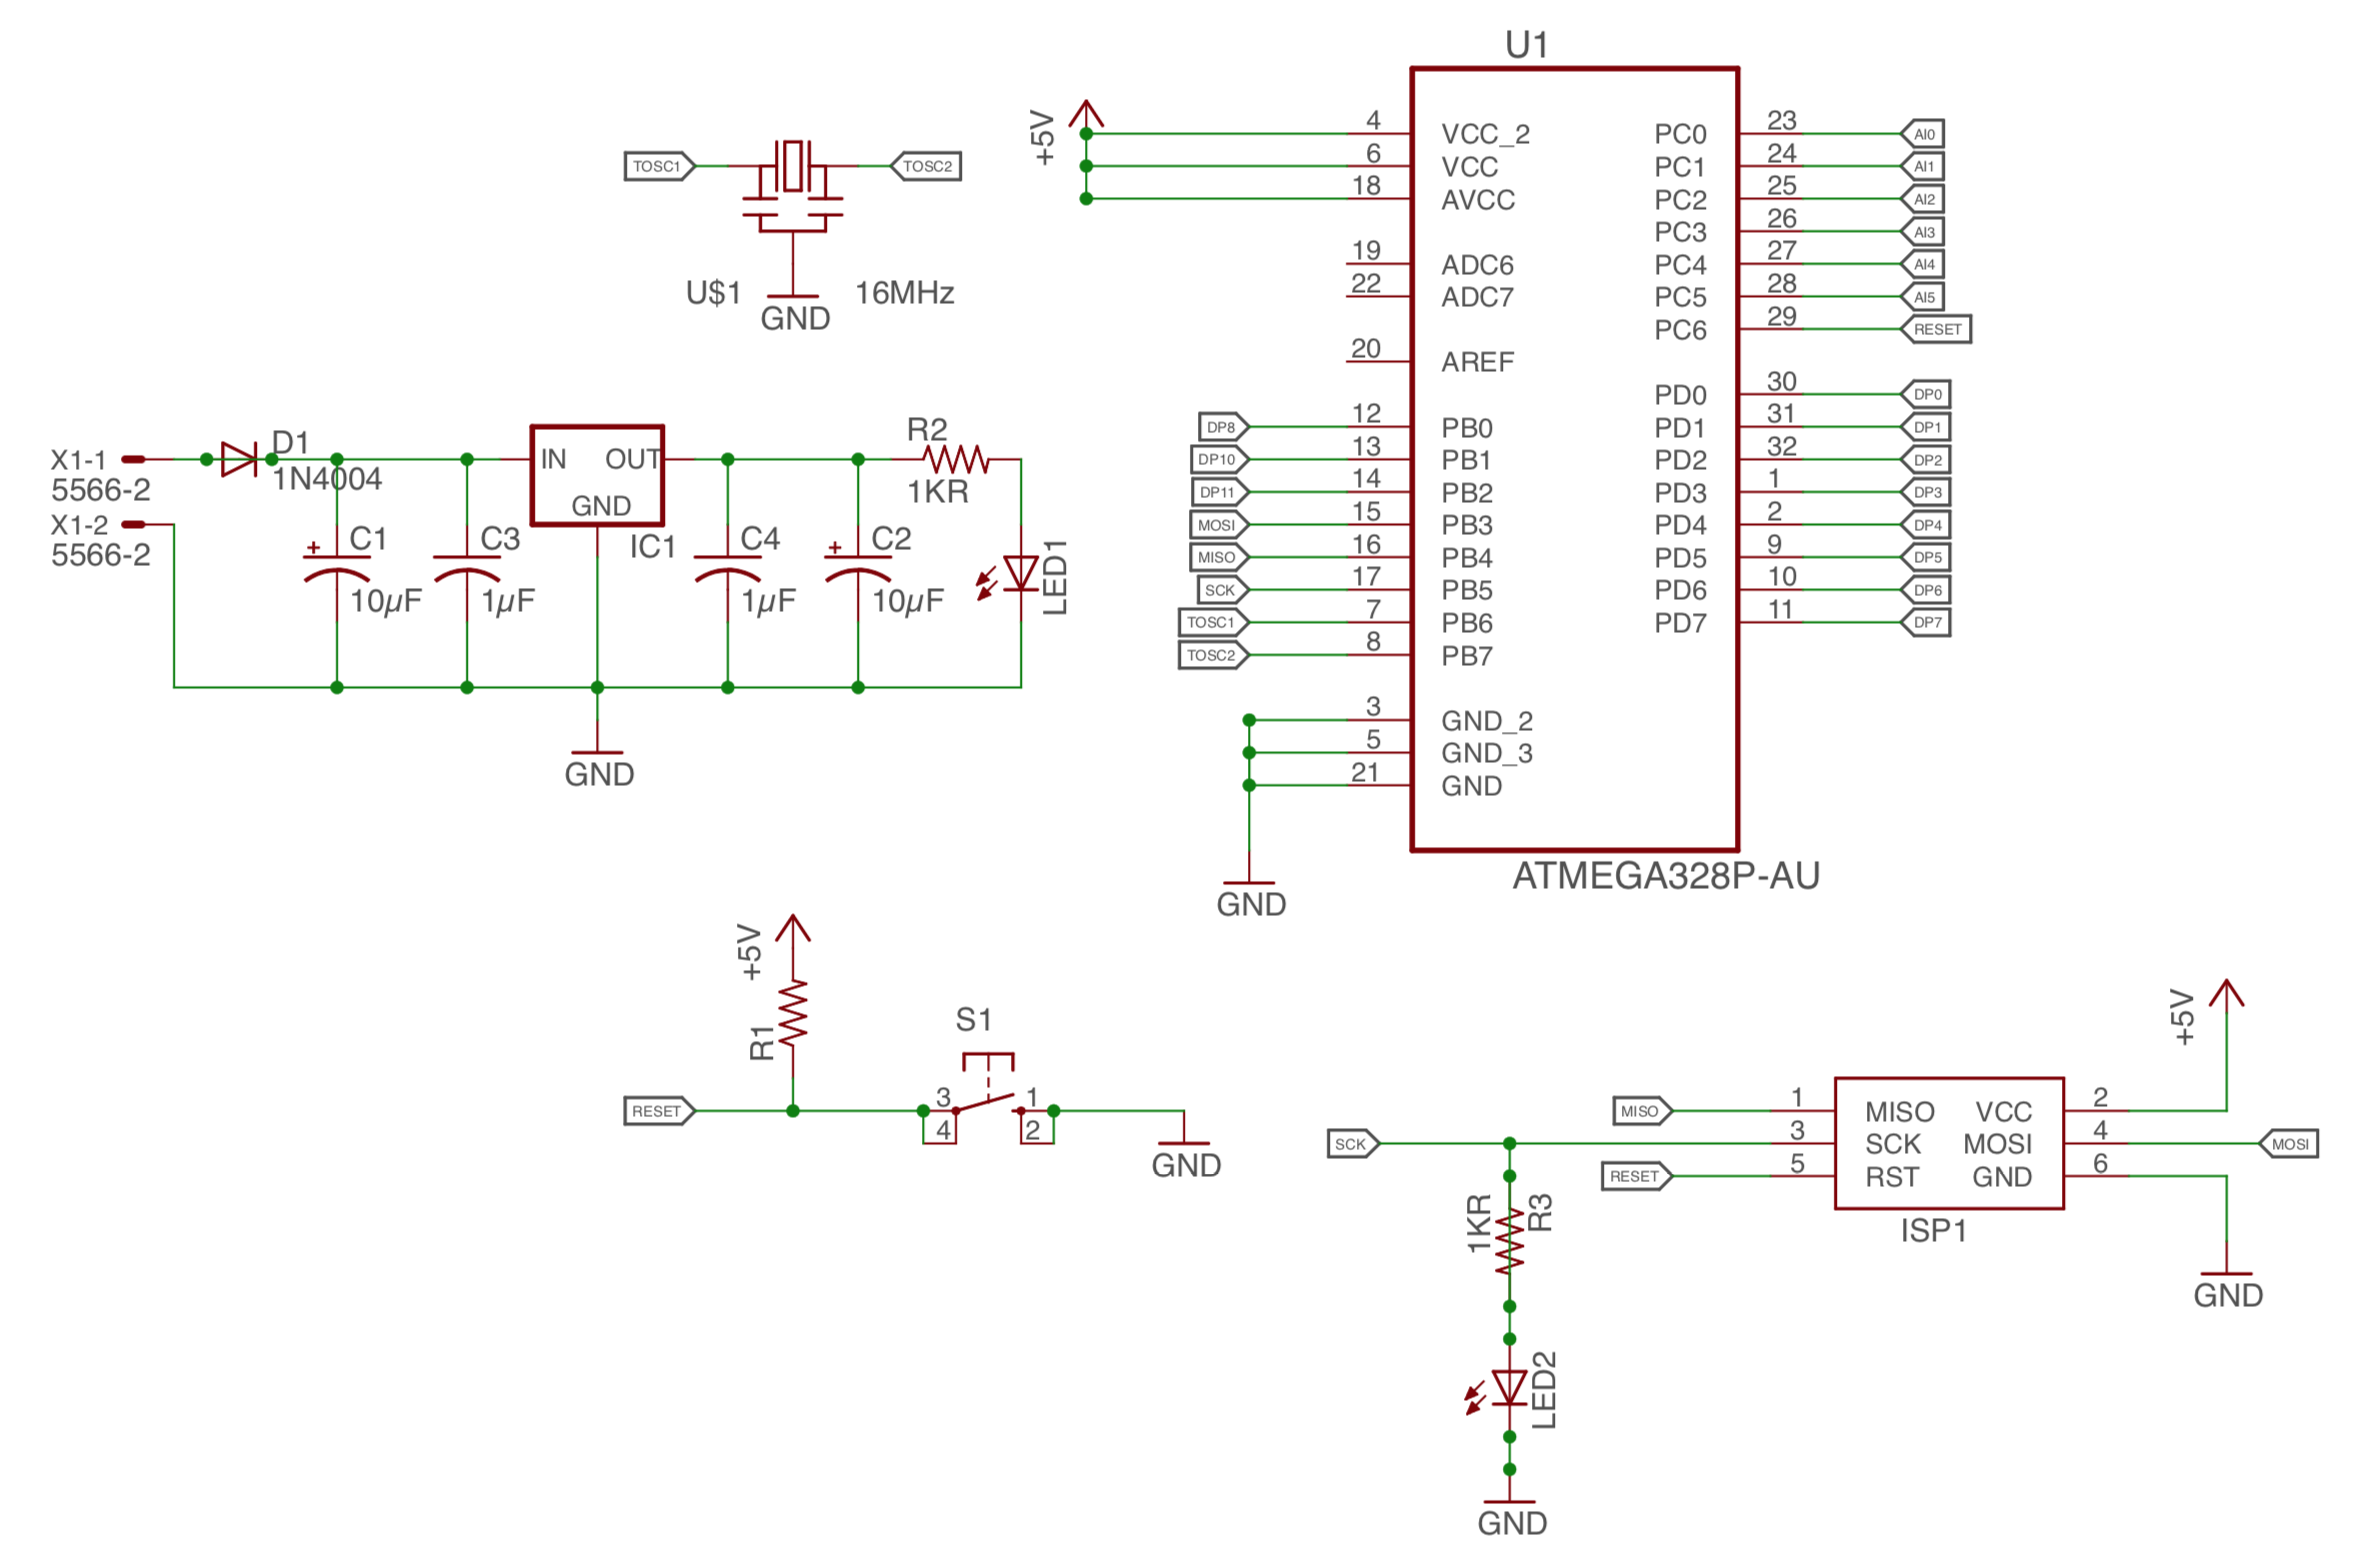
\includegraphics[scale=0.3]{atmega_schemat.png}
    \caption{Schemat}
    \label{fig:my_label}
\end{figure}
%%%%%%%%%%%%%%%%%%%%%%%%%%%%%%%%%%%%%%%STRONA - PODSUMOWANIE
\newpage
\chapter*{Podsumowanie}
Tutaj jakies podusowanie//
Odwołanie do \cite{01}Dziadów. Znowu do \cite{01}dziadów.\\
Teraz do \cite{02} Quo vadi oraz \cite{03} Pana Tadeusza



%%%%%%%%%%%%%%%%%%%%%%%%%%%%%%%%%%%%%%%STRONA - Biblografia
\newpage
\begin{thebibliography}{99}
    \bibitem{01}Adam Mickiewicz - Dziady
    \bibitem{02}Henryk Sienkiewicz - Quo vadis
    \bibitem{03}Adam Mickiewicz - Pan Tadeusz
\end{thebibliography}
%%%%%%%%%%%%%%%%%%%%%%%%%%%%%%%%%%%%%%%STRONA - SPIS RYSUNKOW
\newpage
\listoffigures
%%%%%%%%%%%%%%%%%%%%%%%%%%%%%%%%%%%%%%%STRONA - SPIS TABEL
\newpage
\listoftables
%%%%%%%%%%%%%%%%%%%%%%%%%%%%%%%%%%%%%%%STRONA - SPIS ZALACZNIKOW
\newpage
\chapter*{Spis załączników}

\end{document}
